%!TEX root=main.tex
\section[Aufbau des Auges\hfill Aufbau der Materie]{Aufbau des Auges\\{\normalsize Aufbau der Materie}}
% Das visuelle System dient zur Verarbeitung visueller Information und umfasst Auge, Sehnerv und Teile des Gehirns.

% \subsection{Das Auge}
Das Auge ähnelt in seiner Funktion einer Kamera. Die Linse (Objektiv) sammelt Lichtstrahlen und projiziert diese als auf dem Kopf stehendes gespiegeltes Bild auf die Netzhaut (Film). Da der Abstand zwischen Linse und Netzhaut (Bildweite) unveränderlich ist, muss die Brechkraft (Brennweite) der Augenlinse angepasst werden. Diese Anpassung nennt man \textit{Akkommodation}.

\begin{figure}
	\centering
	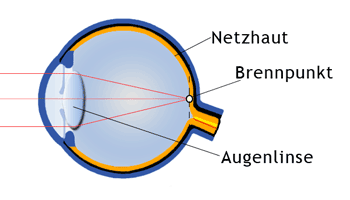
\includegraphics[width=4.5cm]{images/auge.png}
	\caption{Das Auge \cite{auge}}
\end{figure}

Das lichtempfindliche Organ sind die Sehzellen der Netzhaut.